\chapter{Mapas dinámicos}
\label{cap:mapasdinamicos}
En este capítulo se expondrá el sistema creado para la composición de un mapa dinámico que pueda ser usado por paquetes de ROS como \textit{move\_base} o \textit{amcl} y que nos sirva para navegar por el ámbito doméstico de una forma más eficaz y segura de lo que lo haríamos usando un mapa estático o un sistema de \textit{SLAM}.

\section{Arquitectura del sistema}
\label{cap:arquitecturadelsistema}
El sistema propuesto pretende sustituir al nodo map\_server, ya que este nodo solo publica un mapa estático y esto presenta una serie de problemas que veremos más adelante, por tanto nos centramos en esa parte del modelo de navegación de ROS.
\begin{figure} [H]
  \begin{center}
    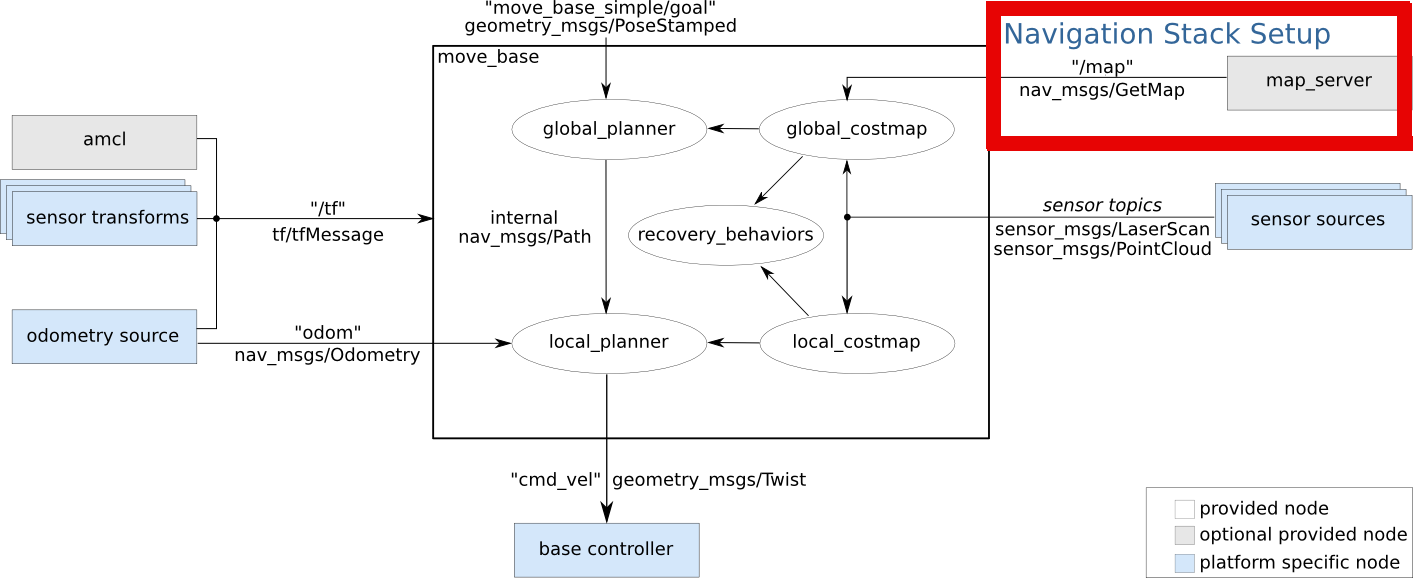
\includegraphics[width=16cm]{img/cap5/navigationstackzoom}
  \end{center}
  \caption{Encuadre de nuestro sistema dentro del modelo de navegación de ROS}
  \label{fig:navigationstackzoom}
\end{figure}

El sistema de mapeado propuesto consta de 3 nodos principales:

\begin{enumerate}
\item Map\_server: Este nodo se encarga de cargar desde fichero el mapa estático y el mapa de largo plazo y activa un servicio para que cualquier otro nodo pueda pedir estos mapas. 
\item Obs\_detector: La función principal de este nodo es la de detectar objetos, leyendo la información proporcionada por el láser, y componer con dicha información el mapa de corto plazo. Para ello solicita los Metadatos de los mapas cargados al nodo Map\_server, creando así un mapa de las mismas medidas y misma resolución que los mapas que maneja el map\_server. Este mapa es publicado para que sea utilizado por el nodo Map\_controller o sea visualizado por la herramienta Rviz.
\item Map\_controller: Nodo que se encarga de la composición del mapa final y de actualizar el mapa de largo plazo con la información obtenida del mapa de corto plazo. Estos mapas son también publicados en distintos topics para que sean utilizados por los nodos encargados de la navegación.
\end{enumerate}
\begin{figure} [H]
  \begin{center}
    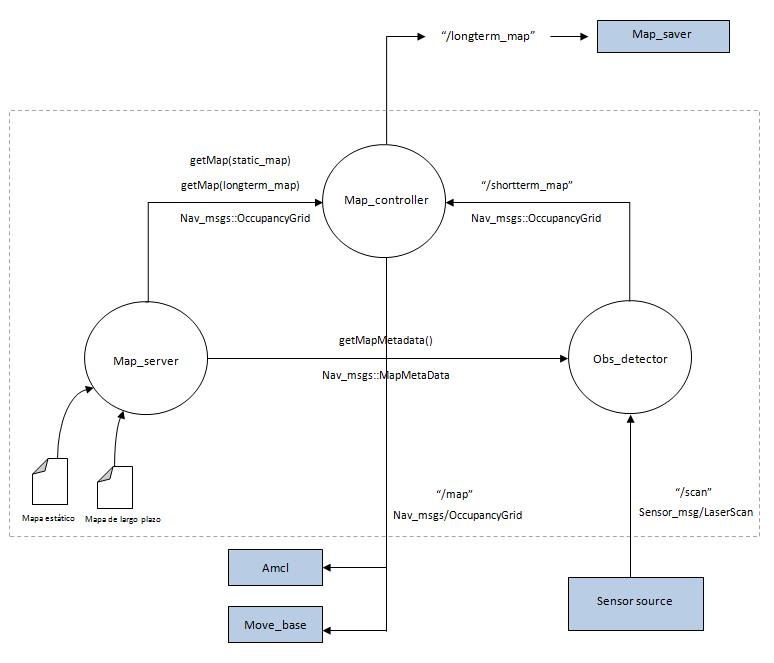
\includegraphics[width=16cm]{img/cap5/esquemaSistema}
  \end{center}
  \caption{Esquema del sistema}
  \label{fig:esquemaSistema}
\end{figure}

\section{Servidor de mapas dinámico}
\label{cap:sevidordemapasdinamico}

En esta sección se describirá el proceso de construcción de los distintos mapas que el servidor de mapas dinámico ofrece, mapa estático, mapa de largo plazo y mapa de corto plazo, así como el proceso de combinación entre ellos para dar lugar al mapa final que será usado por componentes de ROS vistos anteriormente.

\subsection{Mapa estático}
El mapa estático se caracteriza por incluir las partes inmutables del escenario, como son las paredes o las puertas. La mejor manera de construirlo es medir todo el escenario y crear el mapa usando una herramienta de diseño gráfico. En este caso se ha usado \textit{Gimp}.
Este mapa nos servirá como base para crear el mapa de largo plazo.

\begin{figure} [H]
  \begin{center}
    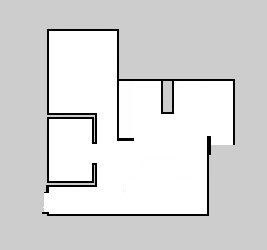
\includegraphics[width=7cm]{img/cap5/mapaestatico}
  \end{center}
  \caption{Mapa estático}
  \label{fig:mapaestatico}
\end{figure}

\subsection{Mapa de corto plazo}
El mapa de corto plazo se caracteriza por ser un mapa en el que se representa los objetos que el robot va percibiendo. Este mapa se inicializa con el valor 255, lo que indica una incertidumbre total. En el instante en el que el algoritmo de construcción del mapa comienza a iterar comenzarán a corregirse estos valores iniciales, asignando el valor 0 a las celdas que corresponden con zonas libres e incrementando desde 0 hasta 254 el valor de las celdas que se perciben como ocupadas.

\renewcommand{\lstlistingname}{Código}
\begin{lstlisting}[caption=Inicialización del cost\_map correspondiente al mapa de corto plazo, label={lst:initcostmap}]

  metadata = getMetadata();
  tf::TransformListener tf(ros::Duration(10));
  cells_size_x = metadata.width;
  cells_size_y = metadata.height;
  resolution = metadata.resolution;
  origin_x = metadata.origin.position.x;
  origin_y = metadata.origin.position.y;
  default_value = 255;
  scan_ready = false;
  pos_ready = false;
  cost_map.resizeMap(cells_size_x,cells_size_y, resolution, origin_x, origin_y);
  cost_map.setDefaultValue(default_value);
  cost_map.resetMap(0,0,cost_map.getSizeInCellsX(), cost_map.getSizeInCellsY());
\end{lstlisting}


El algoritmo propuesto destaca por la capacidad de, no solo añadir objetos al mapa, si no ademas eliminarlos si los objetos desaparecen del lugar que ocupaban. Esto con las herramientas de ROS no puede conseguirse, ya que si solo utilizamos el nodo map\_server para publicar nuestro mapa, tanto el algoritmo de navegación como el de localización cogerán ese mapa y calcularán sobre el nuestra localización y las rutas al destino, pero ese mapa no tendrá en cuenta cambios en el entorno como puede ser una persona paseando por la casa o un mueble cambiado de sitio, es un mapa estático, por lo que puede resultar totalmente erróneo. Por otro lado si usamos la herramienta gmapping para crear nuestro mapa y localizarnos simultáneamente en él, tenemos el mismo problema. En un entorno dinámico con personas moviéndose u objetos cambiando de sitio, se generará un mapa con muchísimo ruido en las zonas libres y con objetos que se mantienen en su lugar cuando ya no están, por lo que la localización empezará a fallar, ya que las muestras del láser no corresponderán con el mapa. 

La solución a este problema se resuelve con la creación de un algoritmo que pueda borrar elementos del mapa. Para ello se compara cada muestra de datos con el mapa que estamos generando y si en dicha muestra existen celdas libres que en el mapa están ocupadas se decrementa el valor de dicha celda en el mapa. La figura \ref{fig:lecturalaser} representa un modelo de una muestra del láser en el que podemos observar lo descrito anteriormente, celdas que marcaremos como ocupadas y celdas que marcaremos como libres. También observamos el límite del láser, que se sitúa en 2.5 metros, a las celdas de mas allá del límite no se les modificará su valor.
La cuantía del decremento se puede modelar, consiguiendo así que el robot olvide más lentamente o más rápidamente los objetos que desaparecen del escenario.

\begin{figure} [H]
  \begin{center}
    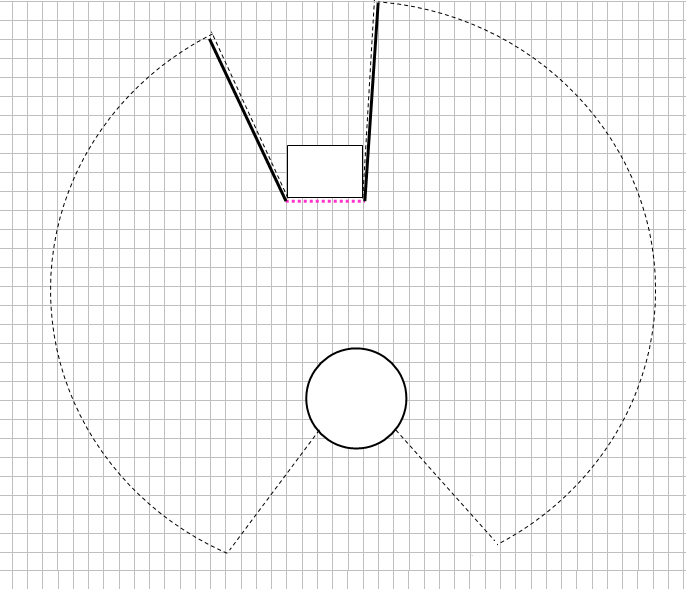
\includegraphics[width=10cm]{img/cap5/lecturaLaser}
  \end{center}
  \caption{Esquematización de una lectura de láser con un objeto.}
  \label{fig:lecturalaser}
\end{figure}


\renewcommand{\lstlistingname}{Código}
\begin{lstlisting}[caption=Función que actualiza el mapa en cada iteración, label={lst:updatecostmap}]
  void
  ObstacleDetector::updateCostmap(){
    if(scan_ready && pos_ready){
      incrementCostProcedure();
      decrementCostProcedure();
    }
    pVectorList_.clear();
    pointList_.clear();
  }
\end{lstlisting}

El proceso de añadir o eliminar un objeto puede ser más o menos rápido dependiendo de los valores de las variables que modelan estas operaciones. Para el caso de nuestro algoritmo contamos un fichero con extensión yaml en el que modificamos los valores de los parámetros.
\renewcommand{\lstlistingname}{Código}
\begin{lstlisting}[caption=Fichero de configuración obstacle\_detector.yaml, label={lst:obstacledetectorconfig}]
  cost_inc: 4
  cost_dec: 1
  min_lenght: 0.23
  max_lenght: 2.5
\end{lstlisting}
Los valores asociados a cost\_inc y cost\_dec representan el incremento o decremento del valor de una celda por cada iteración del algoritmo. Los otros valores configurables representan la longitud máxima y mínima que se tiene en cuenta para cada medida que el láser nos proporciona.

Al final de cada iteración del algoritmo el mapa de corto plazo es publicado en un topic para que pueda ser usado por el resto de nodos que conforman el servidor de mapas dinámico. Para llevar a cabo esta operación usamos una estructura de datos proporcionada por ROS, \textit{Costmap2DPublisher}\footnote{http://docs.ros.org/indigo/api/costmap\_2d/html/classcostmap\_\_2d\_1\_1Costmap2DPublisher.html}. Este publicador publica nuestro mapa en el topic \textit{/shortterm\_map}.


\renewcommand{\lstlistingname}{Código}
\begin{lstlisting}[caption=Step del nodo obstacle\_detector, label={lst:stepobstacledetector}]
  void
  ObstacleDetector::step(){
    updateCostmap();
    cost_map_publisher_.publishCostmap();
  }

  int
  main(int argc, char** argv)
  {
    ros::init(argc, argv, "obstacle_detector");   //Inicializa el nodo
    ObstacleDetector obs;
    ros::Rate loop_rate(5);

    while (ros::ok()){
      obs.step();
      ros::spinOnce();
      loop_rate.sleep();
    }
    return 0;
  }

\end{lstlisting}

Existe un pequeño cambio en los valores del mapa que se publica. El tipo de mensaje que se usa para publicar un costmap es \textit{nav\_msgs::OccupancyGrid}\footnote{http://docs.ros.org/indigo/api/nav\_msgs/html/msg/OccupancyGrid.html}. Este tipo de mensaje contiene, ademas de los metadatos asociados al mapa, un array de datos que representa al mapa. La principal diferencia con un costmap es que los valores en un OccupancyGrid van de 0 a 100 y -1 para las celdas desconocidas ,y no de 0 a 255 como en un costmap.

\subsection{Mapa de largo plazo}
El mapa de largo plazo se inicializa con los valores del mapa estático y se caracteriza por incluir los objetos que tienen un valor muy alto en el mapa de corto plazo, por tanto tenemos un mapa con objetos que han perdurado en el mapa a corto plazo durante un largo periodo de tiempo y que podemos considerar que nos van a influir a la hora de planificar nuestra ruta por el escenario. 
Este mapa también es dinámico, por lo que también elimina los objetos del mapa si estos desaparecen o cambian su posición.


\begin{lstlisting}[caption=Procedimiento para añadir un objeto al mapa de largo plazo, label={lst:addobjectlongmap}]
  void
  MapController::updateLongTermMap(nav_msgs::OccupancyGrid s_map){
    for(int i = 0;i<s_map.data.size();i++){
      if(s_map.data[i] > 95){
        longTerm_map.data[i] = s_map.data[i]; 
        .
        .
        .
      }
    }
  }

\end{lstlisting}

En el código mostrado en \ref{lst:addobjectlongmap} muestra el proceso de adición de un objeto al mapa de largo plazo. Para ello se recorren los valores del mapa de corto plazo y si alguno tiene un valor mayor a 95, valor que consideramos lo suficientemente alto como para que sea muy fiable que esa celda está ocupada, se incluye con ese valor al mapa.

\begin{lstlisting}[caption=Procedimiento para eliminar un objeto al mapa de largo plazo, label={lst:deleteobjectlongmap}]
  void
  MapController::updateLongTermMap(nav_msgs::OccupancyGrid s_map){
    for(int i = 0;i<s_map.data.size();i++){
      .
      .
      .
      }else if(s_map.data[i] < 5 && s_map.data[i] >= 0 && longTerm_map.data[i] >= longterm_cost_dec && static_map.data[i] < 95){
        longTerm_map.data[i] = longTerm_map.data[i] - longterm_cost_dec;
      }
    }
  } 

\end{lstlisting}

En el código mostrado en \ref{lst:deleteobjectlongmap} se compara el mapa de largo plazo con el mapa de corto plazo. Si una celda en el mapa de largo plazo tiene un valor que indica que está ocupada y en el mapa de corto plazo esa misma celda tiene un valor que indica que está libre, siempre y cuando esa celda no pertenezca a una celda de una pared, se decrementa su valor en el mapa de largo plazo. La cuantía de este decremento también puede modelarse, longterm\_cost\_dec, regulando así la memoria que tenemos de los objetos que hemos añadido a este mapa.\pagebreak

Por último publicamos el mapa en el topic \textit{/longTerm\_map}.

\begin{lstlisting}[caption=Publicación del mapa de largo plazo, label={lst:longmappublish}]
longTermMap_pub   = nh_.advertise<nav_msgs::OccupancyGrid>("/longTerm_map", 5); 

void
MapController::publishAll(){
  .
  .
  .
  longTerm_map.header.stamp = ros::Time::now();
  longTermMap_pub.publish(longTerm_map);
}
\end{lstlisting}


Adicionalmente este mapa se guarda cada cierto tiempo en un fichero, usando el nodo por defecto de ROS para este fin ,\textit{map\_saver}\footnote{http://wiki.ros.org/action/fullsearch/map\_server\#map\_saver}. Así por ejemplo podemos tener un cuenta una mesa dentro del salón de una casa para una futura ejecución del algoritmo. Esto nos permitiría planificar una ruta mejor para la navegación, ya que podríamos esquivar esta mesa con facilidad y llegar a nuestro destino lo más rápido posible. Si no tuviéramos esta mesa en cuenta el algoritmo podría planificar una ruta a través de las celdas ocupadas por la mesa. Seguramente el robot no llegaría a chocar, ya que el planificador de rutas usa un pequeño mapa local para evitar estos problemas, pero es seguro que tardaría más en alcanzar su destino ya que al encontrarse frente a la mesa el robot se pararía y tendría que recalcular una nueva ruta. 



\section{Construcción del mapa final}
\label{sec:construccionmap}
El mapa final será la composición de los mapas de largo plazo, que ya incluye el mapa estático, y de corto plazo. Este mapa será usado por el nodo de la navegación y por el nodo de la localización para navegar y localizar al robot en el escenario. La composición del mapa final o mapa efectivo será el resultado de la operación de máximo entre los mapas de corto y de largo plazo, como vemos en el código del apartado \ref{lst:buildEffectivemap}. De esta manera incluiremos en el mapa final toda la información relacionada con los objetos que llevan un tiempo en la escena y también incluiremos, aunque con un menor valor, personas o cosas que acaban de entrar en las inmediaciones del robot.
\pagebreak

\begin{lstlisting}[caption=Composición del mapa final, label={lst:buildEffectivemap}]
  void
  MapController::buildEffectiveMap(nav_msgs::OccupancyGrid s_map,nav_msgs::OccupancyGrid l_map){
    for(int i = 0;i<s_map.data.size();i++){
      effective_map.data[i] = std::max(s_map.data[i],l_map.data[i]);
    }
  }
\end{lstlisting}

Tras la creación del mapa este es publicado en el topic \textit{/map}. 

\begin{lstlisting}[caption=Publicación del mapa final, label={lst:effectivemappublish}]
effectiveMap_pub = nh_.advertise<nav_msgs::OccupancyGrid>("/map", 5);

void
MapController::publishAll(){
  effective_map.header.stamp = ros::Time::now();
  effectiveMap_pub.publish(effective_map);
  .
  .
  .
}
\end{lstlisting}


\subsubsection{Mapeado de zonas desconocidas}
La creación de un mapa de corto plazo a partir de las muestras del láser y la posterior incorporación del mapa de largo plazo para generar un mapa conjunto cuenta con una gran versatilidad y eficacia, tanto que es posible mapear nuevas zonas o estancias del escenario. Generar un mapa así nos permite también localizarnos en este e incluso navegar por el. 

No contamos con un sistema de SLAM, ya que partimos de unos mapas, pero poder incluir en un mapa objetos o nuevas estancias nos permite mantener nuestro robot doméstico por mucho más tiempo navegando por nuestra casa, lo que lo hace mucho más robusto y versátil. Esta ventaja podría, por ejemplo, aplicarse a un robot sirviente en una universidad. Al principio, como prueba de la tecnología, puede que nos interese darle una pequeña zona mapeada por la que moverse, pero si un día queremos que su rango de efectividad se amplíe solo tendremos que moverlo por la zona deseada y se añadirá al mapa perfectamente.


